%==================================
% SMDS TEMPLATE — Data Mining Manuscript (Team LogLoss, UNITY#14), English version
%==================================
\documentclass[11pt,twoside]{article}

%==================================
% PACKAGES
%==================================
\usepackage{amsmath,amssymb}
\usepackage[T1]{fontenc}
\usepackage{graphicx}
\usepackage{geometry}
\geometry{margin=1in}
\usepackage[
backend=biber,
style=numeric-comp,
sorting=none,
giveninits=true,
doi=true,
url=false
]{biblatex}
\addbibresource{SMDSBib.bib}
\usepackage{fancyhdr}
\usepackage{booktabs}
\usepackage{array}
\usepackage{tikz}
\usetikzlibrary{positioning,arrows.meta,calc}
\newcommand{\shorttitle}{}
\newcommand{\shortauthor}{}
\pagestyle{fancy}
\fancyhf{}
\fancyhead[L]{\small\shorttitle}
\fancyhead[R]{\small\shortauthor}
\fancyfoot[C]{\small\thepage}

\usepackage[colorlinks=true,allcolors=blue]{hyperref}
\setlength{\emergencystretch}{2em}
\renewcommand{\abstractname}{Abstract}
\date{19 November 2026}
\newcommand{\orcidlink}[1]{%
\href{https://orcid.org/#1}{
\includegraphics[height=1.6ex]{ORCID_iD.png}}%
}

%==================================
% SIMPLE SMDS MACROS (Compatibility Layer)
%==================================

\newcommand{\SMDStitle}[1]{\title{\bfseries #1}}
\newcommand{\SMDSshorttitle}[1]{\def\shorttitle{#1}}
\newcommand{\SMDSshortafill}[1]{\def\shortauthor{#1}}

\newcommand{\SMDSaffilone}[1]{\def\affilone{#1}}

\newcommand{\SMDSauthorone}[4]{\def\authorone{#1$^{#2}$\,\orcidlink{#3}}}
\newcommand{\SMDSauthortwo}[4]{\def\authortwo{#1$^{#2}$\,\orcidlink{#3}}}
\newcommand{\SMDSauthorthree}[4]{\def\authorthree{#1$^{#2}$\,\orcidlink{#3}}}

\newcommand{\SMDSauthorfour}[4]{\def\authorfour{#1$^{#2}$\,\orcidlink{#3}}}

\newcommand{\SMDScorrespoding}[2]{%
\def\corrauthor{#1 \href{mailto:#2}{#2}}}

\newcommand{\SMDSKeywords}[1]{
\vspace{0.5em}
\noindent\textbf{Keywords:} #1
}

%==================================
% METADATA
%==================================

\SMDStitle{Forecasting the Impact of a Potential 2026 Godzilla El Ni\~no on National Drought in Indonesia Using XGBoost with Spatio-Temporal Kinematic Feature Engineering}

\SMDSshortafill{D. P. Akrilian et al.}
\SMDSshorttitle{ENSO and National Drought in Indonesia}

\SMDSaffilone{Department of Statistics and Data Science, Faculty of Mathematics and Natural Sciences, Universitas Negeri Semarang, Semarang, Indonesia}

%---------------------------------
% AUTHORS
%---------------------------------
\SMDSauthorone{Dimas Pasha Akrilian}{1}{0009-0005-6037-3591}{dimaspasha49@gmail.com}
\SMDSauthortwo{Shata Alwan Jalaluddin}{1}{0009-0007-2139-2487}{}
\SMDSauthorthree{Galih Kusuma Wijaya}{1}{0009-0002-7322-4681}{}
\SMDSauthorfour{M Irfan Al Hakim}{1}{0009-0005-1222-7960}{}

\SMDScorrespoding{$^*$Corresponding author, email:}{dimaspasha49@gmail.com}

%==================================
% AUTHOR BLOCK
%==================================

\author{
\begin{minipage}{\dimexpr\textwidth-12pt\relax}
\authorone,
\authortwo,
\authorthree,
\authorfour
\\[1em]
$^1$ \affilone\\
\corrauthor
\end{minipage}
}

%==================================

\begin{document}

\maketitle

%==================================
\begin{abstract}
\sloppy
Drought early-warning systems often rely on El Ni\~no--Southern Oscillation (ENSO) indicators, yet how far ENSO actually predicts national drought in Indonesia is rarely tested with an evaluation free of target leakage. We analyze 312 monthly observations (2000--2025) that combine CHIRPS, MODIS (NDVI and LST), NOAA OISST, and the Oceanic Ni\~no Index (ONI), with the Standardized Drought Condition Index (SDCI) as the target. In the initial design, XGBoost with 72 features reached a test $R^2$ of 0.80, but those features included same-month NDVI, LST, and rainfall, which are the components that build the SDCI. A linear regression on these three alone gives a test $R^2$ of 1.000, so that figure is not predictive skill. After removing the components and lagging ENSO features by three months, XGBoost tuned by random search with walk-forward validation reaches a test $R^2$ of only 0.070 over 2021--2025, against $-0.051$ for monthly climatology. The strongest cross-correlation is always at lead zero (between $-0.14$ and $-0.34$ depending on region) and vanishes at leads of three months or more; the ONI regression coefficient is significant only at leads of 0 and 1 month, and Granger tests are not significant at the 5\% level. The same-month effect is strongest in Java and Nusa Tenggara. Under a scenario in which ONI rises linearly by 0.15 per month, the national SDCI is lowest in September 2026 at 0.399 (10--90\% range 0.36--0.54), below the historical September mean (0.493) and above the critical threshold of 0.3, although the model is not shown to beat climatology. ENSO is therefore more useful for concurrent monitoring than for three-month-ahead forecasting, and all results are reproducible with a fixed seed.

\end{abstract}

\SMDSKeywords{ENSO, drought, SDCI, XGBoost, target leakage, walk-forward validation, Godzilla El Ni\~no}

%==================================
\section{Introduction}
\label{Sec:Intro}

El Ni\~no-driven drought has repeatedly strained agriculture and triggered land fires in Indonesia. Indonesian rainfall is strongly tied to tropical Pacific sea surface temperature and local air--sea interaction \cite{hendon2003indonesian,aldrian2003rainfall,hamada2002rainy}, and the 2015 fires and smoke showed that El Ni\~no-induced drought can act nonlinearly on peatland \cite{field2016fire}. The 2015/2016 event was an extreme El Ni\~no that differed in character from 1997/1998 \cite{paek2017different}. The label ``Godzilla El Ni\~no'' is used for a very strong El Ni\~no, and the prospect of a similar event in 2026 raises a practical question: how early and how well can national drought be warned of from ENSO indicators?

Machine learning is increasingly used for climate forecasting, including ENSO itself \cite{ham2019deep}, and tree-based models such as XGBoost \cite{chen2016xgboost} are popular for their accuracy on tabular data. High accuracy on time series, however, is easily misleading. Target leakage, meaning features that carry information about the target that would not be available at prediction time, is among the most common errors that inflate model scores \cite{kaufman2012leakage}, and cross-validation that shuffles time order compounds the problem \cite{bergmeir2012cv}. For a composite index such as the SDCI, built from NDVI, land surface temperature, and rainfall \cite{rhee2010sdci,kogan1995vci}, using those components as predictors is equivalent to putting the answer in the question.

This study began with an early-warning system based on XGBoost and climate-kinematics feature engineering (ONI momentum and acceleration) whose initial version reported a test $R^2$ of 0.83. While auditing its feature pipeline we found that this figure came from the components of the SDCI. This article reports that finding and answers the original question again with a leakage-free design. The article makes three contributions. First, we demonstrate the target leakage quantitatively and show that $R^2$ falls from 0.80 to 0.07 once it is fixed. Second, we measure the lead--lag structure between ONI and the SDCI nationally and by region with inference that is robust to autocorrelation (Newey--West errors \cite{newey1987hac}) and Granger tests \cite{granger1969causality}. Third, we compare tuned XGBoost with simple benchmarks, namely monthly climatology and classical time-series models, in out-of-sample evaluation, and find that the ENSO model does not beat climatology at a three-month lead.

Section~\ref{Sec:Related} reviews related work. Section~\ref{Sec:Method} describes the data, feature engineering, leakage-free design, and modeling. Section~\ref{Sec:Results} reports the results, Section~\ref{Sec:Discussion} discusses them together with their limitations, and Section~\ref{Sec:Conclusion} concludes.

%==================================
\section{Related Work}
\label{Sec:Related}

\paragraph{ENSO and Indonesian rainfall.} Hendon \cite{hendon2003indonesian} showed that ENSO modulates Indonesian rainfall, with a prominent effect in the dry season and local air--sea interaction amplifying the signal. Aldrian and Susanto \cite{aldrian2003rainfall} divided Indonesia into three dominant rainfall regions with different relationships to sea surface temperature, and Hamada et al.\ \cite{hamada2002rainy} linked variations in the onset and end of the rainy season to ENSO. The regional heterogeneity we find agrees with this picture, although we use a drought index built from remote sensing rather than rainfall alone.

\paragraph{Satellite-based drought indices.} Indices such as the Vegetation Condition Index \cite{kogan1995vci} and composite indices that combine vegetation, temperature, and rainfall \cite{rhee2010sdci} are widely used to monitor agricultural drought. Because the index is a composite, its components cannot serve as predictors of the same index.

\paragraph{Machine learning and time-series validation.} XGBoost \cite{chen2016xgboost}, LightGBM \cite{ke2017lightgbm}, and Random Forest \cite{breiman2001rf} are often compared with classical time-series models and Prophet \cite{taylor2018prophet}. For time series, Bergmeir and Ben\'itez \cite{bergmeir2012cv} discuss when cross-validation is valid, while Hyndman and Athanasopoulos \cite{hyndman2021fpp3} stress simple benchmarks and out-of-sample evaluation. Skill scores against climatology follow Murphy \cite{murphy1988skill}. Hyperparameters are tuned by random search over the Optuna \cite{akiba2019optuna} search space, and model explanations use SHAP values \cite{lundberg2017shap}. We add a case study showing how large leakage can be for a composite index and what it does to the conclusions.

%==================================
\section{Methodology}
\label{Sec:Method}

Figure~\ref{Fig:Pipeline} summarizes the workflow. The statistical analysis is done in R (cross-correlation, lead regression, Granger tests) and so is the machine-learning modeling (XGBoost, benchmarks, and the 2026 scenario). Every step is run with a fixed seed.

\begin{figure}[ht]
\centering
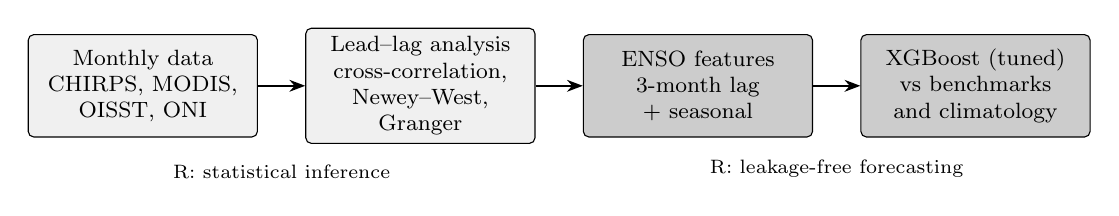
\begin{tikzpicture}[
  box/.style={draw, rounded corners=2pt, align=center, font=\footnotesize, text width=2.7cm, minimum height=13mm, inner sep=3pt},
  stat/.style={box, fill=black!6},
  ml/.style={box, fill=black!20},
  arr/.style={-{Stealth[length=2mm]}, thick},
  node distance=6mm]
\node[stat] (a) {Monthly data\\CHIRPS, MODIS,\\OISST, ONI};
\node[stat, right=of a] (b) {Lead--lag analysis\\cross-correlation,\\Newey--West, Granger};
\node[ml, right=of b] (c) {ENSO features\\3-month lag\\+ seasonal};
\node[ml, right=of c] (d) {XGBoost (tuned)\\vs benchmarks\\and climatology};
\draw[arr] (a)--(b); \draw[arr] (b)--(c); \draw[arr] (c)--(d);
\node[font=\scriptsize] at ($(a.south)!0.5!(b.south)+(0,-4mm)$) {R: statistical inference};
\node[font=\scriptsize] at ($(c.south)!0.5!(d.south)+(0,-4mm)$) {R: leakage-free forecasting};
\end{tikzpicture}
\caption{Research workflow. Light boxes are statistical analysis (R); dark boxes are machine-learning modeling (also R).}
\label{Fig:Pipeline}
\end{figure}

\subsection{Data}
\label{SubSec:Data}

The data consist of 312 monthly observations, January 2000 to December 2025, with 40 numeric variables acquired through Google Earth Engine (Table~\ref{Tab:Data}). Each land variable is available for Indonesia as a whole and for seven regional groups: Sumatra, Java, Kalimantan, Sulawesi, Nusa Tenggara, Maluku, and Papua. The target is the national SDCI (\texttt{SDCI\_Indo}), a composite of the Vegetation Condition Index (VCI), Temperature Condition Index (TCI), and Precipitation Condition Index (PCI) scaled to 0--1; small values indicate drought and the critical threshold used is 0.3. A total of 38 missing cells (0.3\% of 12,480 cells) were filled by time-aware interpolation.

\begin{table}[ht]
\centering
\caption{Data sources. All series are monthly, 2000--2025 (312 observations).}
\label{Tab:Data}
\small
\begin{tabular}{llp{6.2cm}}
\toprule
Source & Variables & Notes \\
\midrule
CHIRPS \cite{funk2015chirps} & rainfall & by region and national \\
MODIS & NDVI, LST & vegetation index and land surface temperature, by region \\
NOAA OISST \cite{huang2021oisst} & SST, \textit{sst\_anomaly}, Ni\~no 1+2/3.4/4 & sea surface temperature and anomaly \\
NOAA & ONI \cite{trenberth1997enso} & Ni\~no 3.4 SST anomaly, three-month running mean \\
Derived & regional SDCI & from VCI, TCI, and PCI \\
\bottomrule
\end{tabular}
\end{table}

Climate phases are set from ONI with thresholds of $\pm 0.5$: 81 La Ni\~na months, 161 neutral, and 70 El Ni\~no. The national SDCI averages 0.620 (standard deviation 0.115) and only five months fall below 0.3.

\subsection{Seasonal anomalies and lead--lag analysis}
\label{SubSec:LeadLag}

The SDCI is strongly seasonal: monthly means explain 58.9\% of its variance, with the lowest value in October (0.462) and the highest in May (0.744). To keep seasonality from masking the relationship with ONI, we use the anomaly $A_t = \mathrm{SDCI}_t - \overline{\mathrm{SDCI}}_{m(t)}$, the difference from the climatology of the same calendar month. Three analyses are run on this anomaly.

\paragraph{Cross-correlation.} We compute $\mathrm{corr}(\mathrm{ONI}_t, A_{t+h})$ for $h = 0,\dots,12$ months, by region.

\paragraph{Lead regression.} For the national SDCI, $A_{t+h} = \alpha_h + \beta_h\,\mathrm{ONI}_t + \varepsilon_{t+h}$ with $h = 0,\dots,9$. Standard errors use the Newey--West estimator \cite{newey1987hac} with a Bartlett kernel and lag 12, without prewhitening, because errors are strongly autocorrelated in monthly data.

\paragraph{Granger test.} We test whether ONI helps predict $A_t$ beyond the history of $A_t$ itself \cite{granger1969causality} with orders 3, 6, and 9. This test measures predictive content, not physical causation.

\subsection{Climate-kinematics feature engineering}
\label{SubSec:Features}

From ONI and \textit{sst\_anomaly} we build 21 features per variable: the raw value, lags of 1--6 and 12 months, rolling mean, standard deviation, maximum, and minimum (windows of 3 and 6 months), exponential moving averages (spans 3 and 6), and the kinematic features
\begin{equation}
v_t = x_t - x_{t-1}, \qquad v^{(3)}_t = x_t - x_{t-3}, \qquad a_t = v_t - v_{t-1},
\label{Eq:Kinematic}
\end{equation}
called momentum (rate of change) and acceleration, intended to capture the onset of rapid Pacific warming. Two seasonal features, $\sin(2\pi m/12)$ and $\cos(2\pi m/12)$, are added. The result is 44 features.

\subsection{Leakage-free design}
\label{SubSec:Leakfree}

The initial version of the study used 72 features: the ENSO features above plus all land variables (NDVI, LST, rainfall, \textit{Suhu\_Permukaan\_C}, \textit{Curah\_Hujan\_mm}) in the same month as the target. Because the SDCI is built from NDVI, LST, and rainfall, that design leaks the target. The leakage-free design follows three rules.
\begin{enumerate}
\item Variables that build the SDCI are not used in the target month. Predictors are only ONI and \textit{sst\_anomaly} features lagged by $H = 3$ months, that is, features up to month $t - 3$ predict the SDCI of month $t$, plus two seasonal features that are known for the target month.
\item The split is chronological 80/20: 237 training months (April 2001--December 2020) and 60 test months (January 2021--December 2025). The test data are not touched during tuning or early stopping, which uses the last 15\% of the training data as validation.
\item All models are compared on the same features and split, and monthly climatology (mean SDCI per calendar month from the training data) is reported as the main benchmark.
\end{enumerate}

\subsection{Modeling}
\label{SubSec:Models}

XGBoost \cite{chen2016xgboost} with a squared-error objective is tuned by random search (50 trials, seed 42) over the search space used with Optuna \cite{akiba2019optuna}, without pruning. The objective is the mean RMSE over five-fold walk-forward validation (\texttt{TimeSeriesSplit}) inside the training data. The search space covers the number of trees (100--500), depth (3--9), learning rate ($0.005$--$0.1$, log scale), \textit{subsample} and \textit{colsample} (0.5--0.9), minimum child weight (1--10), L1 and L2 regularization ($10^{-3}$--10), and $\gamma$ ($10^{-3}$--1). Benchmarks are ARIMA(1,1,1), Prophet \cite{taylor2018prophet}, Random Forest \cite{breiman2001rf}, LightGBM \cite{ke2017lightgbm}, XGBoost with default parameters, and monthly climatology.

For the 2026 scenario, three quantile XGBoost models (pinball-loss objective \cite{koenker1978quantile} at quantiles 0.1, 0.5, and 0.9) are trained on ONI-derived and seasonal features. The scenario assumes that ONI rises linearly by 0.15 per month over twelve months from its last value (December 2025: $-0.60$). This path is an assumption, not an ONI forecast.

\subsection{Walk-forward validation}
\label{SubSec:WFV}

Because the data are a time series, random K-fold cross-validation would mix future and past months and leak information. Model selection therefore uses walk-forward validation (\texttt{TimeSeriesSplit} with five folds) inside the 237 training months (Figure~\ref{Fig:WFV}). The training window expands from 42 to 198 months starting in April 2001, and each fold is validated on the following 39 months. The test months (2021--2025) belong to no fold. The mean validation RMSE over the five folds is the tuning objective, and the per-fold scores show how stable the model is over time.

\begin{figure}[ht]
\centering
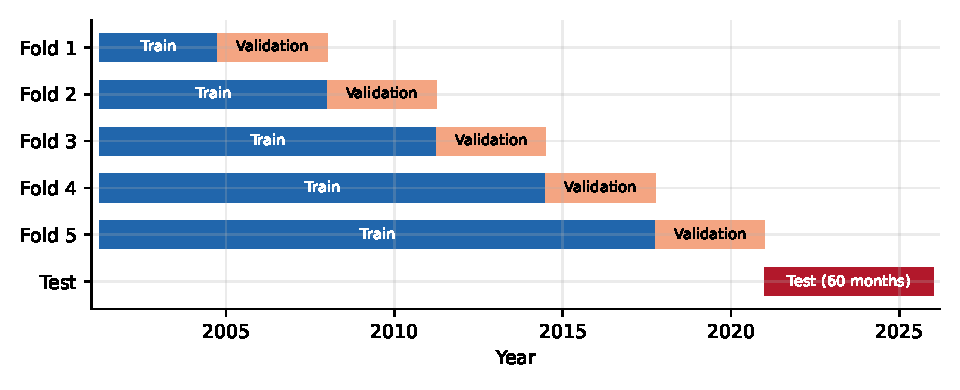
\includegraphics[width=0.85\textwidth]{figs_en/fig_wfv.pdf}
\caption{Walk-forward validation inside the training data (April 2001--December 2020); the test months are never touched.}
\label{Fig:WFV}
\end{figure}

\subsection{Metrics and reproducibility}
\label{SubSec:Metrics}

We report RMSE, MAE, and the test coefficient of determination $R^2 = 1 - \sum (y_t - \hat y_t)^2 / \sum (y_t - \bar y)^2$. For expanding-window out-of-sample evaluation we use the skill score $1 - \mathrm{MSE}_{\mathrm{ONI}} / \mathrm{MSE}_{\mathrm{clim}}$ against climatology \cite{murphy1988skill}, which is positive when the ENSO model beats climatology. All code is run with seed 42 (\texttt{set.seed}); two consecutive renders of the R Markdown document produced identical results.

%==================================
\section{Empirical Results}
\label{Sec:Results}

\subsection{Overview of the SDCI and ONI}
\label{SubSec:Overview}

Figure~\ref{Fig:TS} shows the national SDCI anomaly and ONI. The lowest SDCI of the whole period occurred in October 2015 (0.013), just before ONI peaked in December 2015 (2.62) as the 2015/2016 El Ni\~no developed. The raw correlation between ONI and SDCI is only $-0.19$. Mean SDCI in the El Ni\~no phase (0.568) is lower than in the neutral (0.646) and La Ni\~na (0.614) phases, but its standard deviation is the largest (0.142), so the distributions are wide and overlap.

\begin{figure}[ht]
\centering
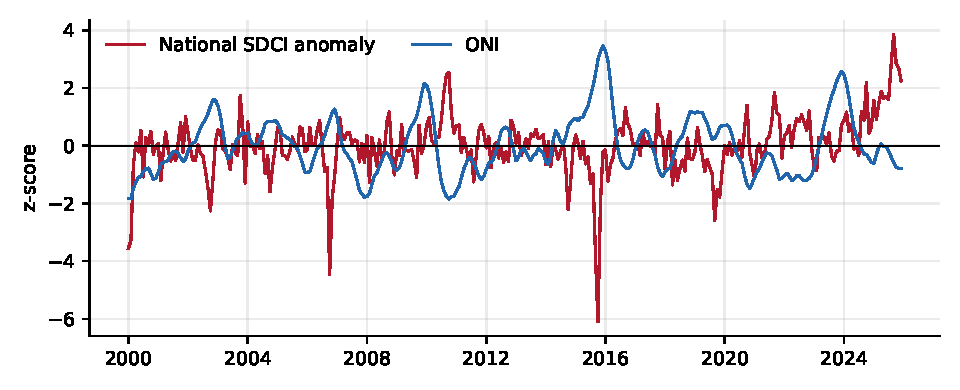
\includegraphics[width=0.85\textwidth]{figs_en/fig_ts.pdf}
\caption{National SDCI anomaly and ONI (both standardized). SDCI drops coincide with strong El Ni\~no, but ONI peaks are not always followed by a proportionate SDCI drop.}
\label{Fig:TS}
\end{figure}

\subsection{Lead--lag structure}
\label{SubSec:Lag}

Figure~\ref{Fig:CC} presents cross-correlation by region. In every region the strongest negative correlation is at lead zero and weakens quickly as the lead grows; there is no evidence of an impact delayed by several months. Values range from $-0.14$ (Papua) to $-0.34$ (Nusa Tenggara); nationally $-0.29$.

\begin{figure}[ht]
\centering
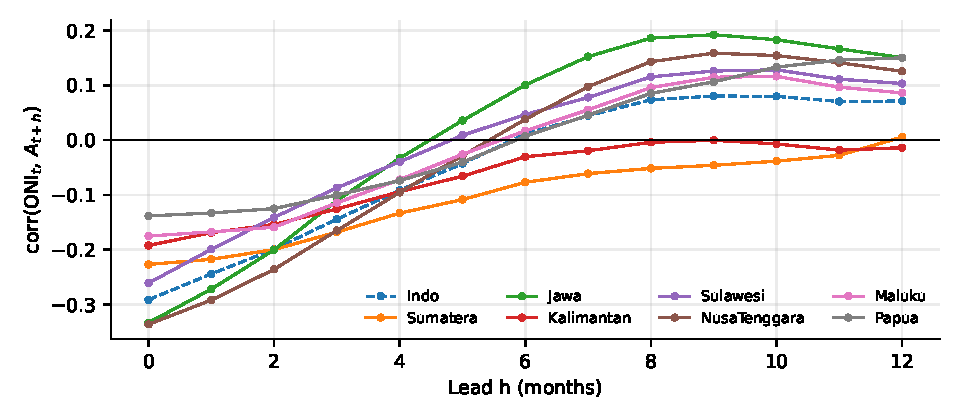
\includegraphics[width=0.85\textwidth]{figs_en/fig_cc.pdf}
\caption{Cross-correlation between ONI in month $t$ and the SDCI anomaly in month $t+h$. The dashed line is the national SDCI.}
\label{Fig:CC}
\end{figure}

Table~\ref{Tab:Lead} and Figure~\ref{Fig:Beta} report the national lead regression. The ONI coefficient is significant at lead 0 ($\hat\beta = -0.028$, $p = 0.021$) and lead 1 ($-0.023$, $p = 0.032$), borderline at lead 2 ($p = 0.053$), and not significant from lead 3 onward. The coefficient changes sign from lead 6, but with a standard error larger than its value. The highest $R^2$ is only 0.085, that is, ONI explains less than a tenth of the variation in the same-month SDCI anomaly. Granger tests are not significant at the 5\% level: $p = 0.091$ (order 3), 0.154 (order 6), and 0.051 (order 9).

\begin{table}[ht]
\centering
\caption{Lead regression of the national SDCI anomaly on ONI: $A_{t+h} = \alpha_h + \beta_h\,\mathrm{ONI}_t$. Newey--West standard errors (lag 12); $n = 312 - h$.}
\label{Tab:Lead}
\small
\begin{tabular}{rrrrr}
\toprule
$h$ (months) & $\hat\beta_h$ & Std.\ error & $p$-value & $R^2$ \\
\midrule
0 & $-0.0282$ & 0.0122 & 0.021 & 0.085 \\
1 & $-0.0232$ & 0.0108 & 0.032 & 0.060 \\
2 & $-0.0186$ & 0.0096 & 0.053 & 0.040 \\
3 & $-0.0135$ & 0.0087 & 0.121 & 0.021 \\
4 & $-0.0086$ & 0.0082 & 0.298 & 0.008 \\
5 & $-0.0040$ & 0.0082 & 0.623 & 0.002 \\
6 & $0.0010$ & 0.0084 & 0.902 & 0.000 \\
7 & $0.0041$ & 0.0088 & 0.640 & 0.002 \\
8 & $0.0069$ & 0.0092 & 0.457 & 0.005 \\
9 & $0.0075$ & 0.0094 & 0.425 & 0.007 \\
\bottomrule
\end{tabular}
\end{table}

\begin{figure}[ht]
\centering
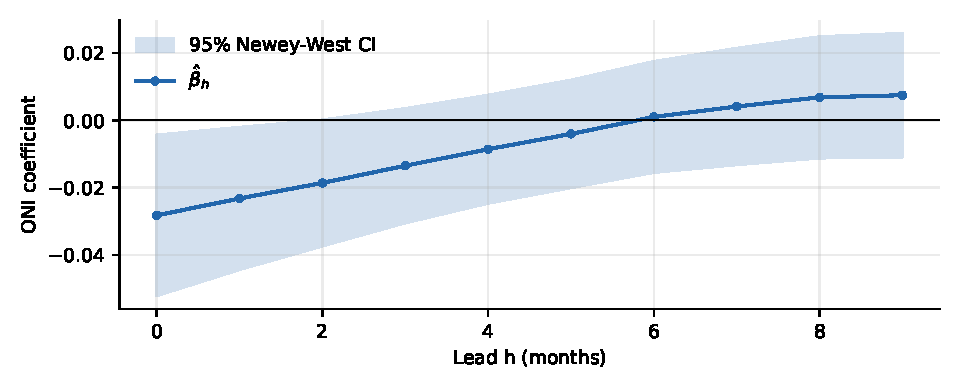
\includegraphics[width=0.85\textwidth]{figs_en/fig_beta.pdf}
\caption{ONI coefficient on the national SDCI anomaly by lead, with a 95\% Newey--West confidence band. The band contains zero from lead 2.}
\label{Fig:Beta}
\end{figure}

\subsection{Regional heterogeneity}
\label{SubSec:Regions}

Table~\ref{Tab:Regions} shows that the lead-zero ONI coefficient is negative in every region, but its strength differs. Nusa Tenggara ($-0.038$, $p = 0.001$) and Java ($-0.035$, $p = 0.0005$) are the most sensitive, with $R^2$ around 0.11. Sulawesi and Sumatra are significant at the 5\% level but not after a Bonferroni correction for eight regions ($\alpha = 0.00625$), while Kalimantan, Maluku, and Papua are not significant. Only Java and Nusa Tenggara remain significant after the correction.

\begin{table}[ht]
\centering
\caption{Lead-0 regression of the regional SDCI anomaly on ONI (Newey--West standard errors). Bonferroni correction for eight regions: $\alpha = 0.00625$.}
\label{Tab:Regions}
\small
\begin{tabular}{lrrr}
\toprule
Region & $\hat\beta_0$ & $p$-value & $R^2$ \\
\midrule
Nusa Tenggara & $-0.0383$ & 0.0010 & 0.113 \\
Java          & $-0.0354$ & 0.0005 & 0.111 \\
Indonesia     & $-0.0282$ & 0.0212 & 0.085 \\
Sulawesi      & $-0.0240$ & 0.0095 & 0.068 \\
Sumatra       & $-0.0207$ & 0.0496 & 0.052 \\
Kalimantan    & $-0.0191$ & 0.1537 & 0.037 \\
Maluku        & $-0.0171$ & 0.1379 & 0.031 \\
Papua         & $-0.0111$ & 0.2058 & 0.019 \\
\bottomrule
\end{tabular}
\end{table}

\subsection{Demonstration of target leakage}
\label{SubSec:Leak}

Figure~\ref{Fig:Leak} and Table~\ref{Tab:Leak} summarize the core experiment. A linear regression of the national SDCI on same-month national NDVI, LST, and rainfall gives a test $R^2$ of 1.000 (chronological 80/20 split on 312 months), meaning the SDCI is an almost deterministic function of the three. When same-month ONI and \textit{sst\_anomaly} are used without those components, the test $R^2$ is $-0.373$. The initial 72-feature design obtained a test $R^2$ of 0.80 with tuned XGBoost, and the initial report even recorded 0.83; both figures reflect only the features that build the SDCI.

\begin{figure}[ht]
\centering
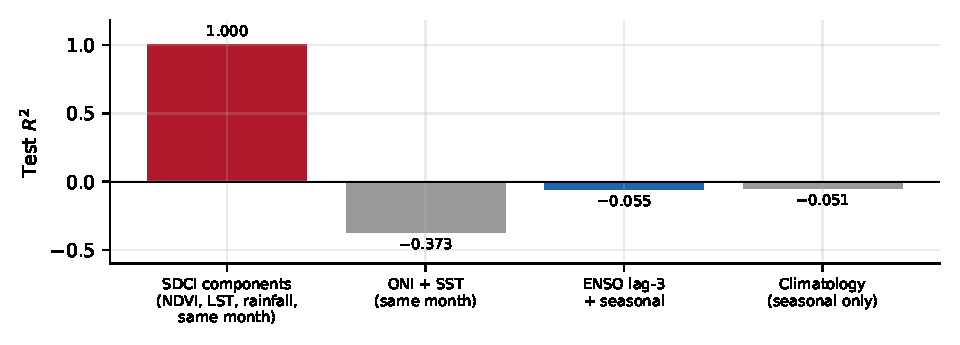
\includegraphics[width=0.85\textwidth]{figs_en/fig_leak.pdf}
\caption{Test $R^2$ of linear models for the national SDCI by predictor set. Same-month SDCI components reconstruct the target almost perfectly, whereas legitimate ENSO predictors do not beat climatology.}
\label{Fig:Leak}
\end{figure}

\begin{table}[ht]
\centering
\caption{Test $R^2$ of linear models for the national SDCI. Rows 1--2: 80/20 split on 312 months (63 test months). Rows 3--4: leakage-free sample with a 3-month lead, 297 months (60 test months, 2021--2025).}
\label{Tab:Leak}
\small
\begin{tabular}{lr}
\toprule
Predictors & Test $R^2$ \\
\midrule
National NDVI, LST, rainfall (same month) & 1.000 \\
ONI + \textit{sst\_anomaly} (same month) & $-0.373$ \\
ENSO 3-month lag + seasonal (OLS) & $-0.055$ \\
Monthly climatology & $-0.051$ \\
\bottomrule
\end{tabular}
\end{table}

\subsection{Expanding-window out-of-sample evaluation}
\label{SubSec:OOS}

To avoid depending on a single split, we evaluate the model $y_t = \alpha + \beta\,\mathrm{ONI}_{t-h} + \gamma_{m(t)}$ recursively: each test month (2021 to 2025) is predicted using only the data pairs available at that time and then compared with climatology. Table~\ref{Tab:OOS} shows a negative skill score at every lead tested (1, 3, 6, and 9 months): adding ONI slightly increases error relative to climatology, with a very small RMSE difference (under 0.001 at lead 3).

\begin{table}[ht]
\centering
\caption{Expanding-window out-of-sample evaluation (test months 2021--2025). Skill score $1 - \mathrm{MSE}_{\mathrm{ONI}}/\mathrm{MSE}_{\mathrm{clim}}$; a negative value means the ONI model is worse than climatology.}
\label{Tab:OOS}
\small
\begin{tabular}{rrrrr}
\toprule
Lead (months) & $n$ test & RMSE ONI+seasonal & RMSE climatology & Skill score \\
\midrule
1 & 62 & 0.0933 & 0.0933 & $-0.0017$ \\
3 & 60 & 0.0869 & 0.0862 & $-0.0173$ \\
6 & 57 & 0.0726 & 0.0724 & $-0.0038$ \\
9 & 54 & 0.0675 & 0.0674 & $-0.0015$ \\
\bottomrule
\end{tabular}
\end{table}

\subsection{XGBoost and benchmarks on leakage-free features}
\label{SubSec:ML}

Table~\ref{Tab:Bench} and Figure~\ref{Fig:Bench} compare all models on the 44 leakage-free features and a three-month lead (60 test months). Tuned XGBoost achieves the best RMSE (0.0935) and a test $R^2$ of 0.070, the only positive value. This is far from the 0.80 of the initial design. LightGBM ($-0.004$), Random Forest ($-0.025$), and climatology ($-0.051$) are around zero, default XGBoost is $-0.214$, Prophet $-0.417$, and ARIMA $-1.099$. The gap between tuned XGBoost and climatology (RMSE 0.0935 versus 0.0993) is small and we did not test its significance; with 60 autocorrelated test months, it is not enough to conclude superiority. The best walk-forward validation RMSE is 0.0698 (trial 22, 354 iterations), against 0.0701 for climatology on the same folds; XGBoost is better on three of five folds and worse on two. Per-fold XGBoost $R^2$ ranges from 0.43 to 0.81 but largely reflects seasonality, since climatology alone reaches 0.12--0.81 on the same folds. The negative $R^2$ values are partly driven by a level shift: mean SDCI in the test period (0.673) is higher than in the training data (0.610), and the test period contains the 2023 El Ni\~no (peak ONI 1.95) with a lowest SDCI of 0.447.

\begin{table}[ht]
\centering
\caption{Test performance (2021--2025, 60 months) on ENSO 3-month-lag + seasonal features. Tuned XGBoost and the benchmarks use the same split and features.}
\label{Tab:Bench}
\small
\begin{tabular}{lrrr}
\toprule
Model & RMSE & MAE & $R^2$ \\
\midrule
XGBoost (tuned)     & \textbf{0.0935} & 0.0708 & \textbf{0.0698} \\
LightGBM            & 0.0971 & 0.0716 & $-0.0036$ \\
Random Forest       & 0.0981 & 0.0768 & $-0.0253$ \\
Monthly climatology & 0.0993 & 0.0746 & $-0.0505$ \\
XGBoost (default)   & 0.1067 & 0.0789 & $-0.2137$ \\
Prophet             & 0.1153 & 0.0908 & $-0.4171$ \\
ARIMA(1,1,1)        & 0.1404 & 0.1189 & $-1.0990$ \\
\bottomrule
\end{tabular}
\end{table}

\begin{figure}[ht]
\centering
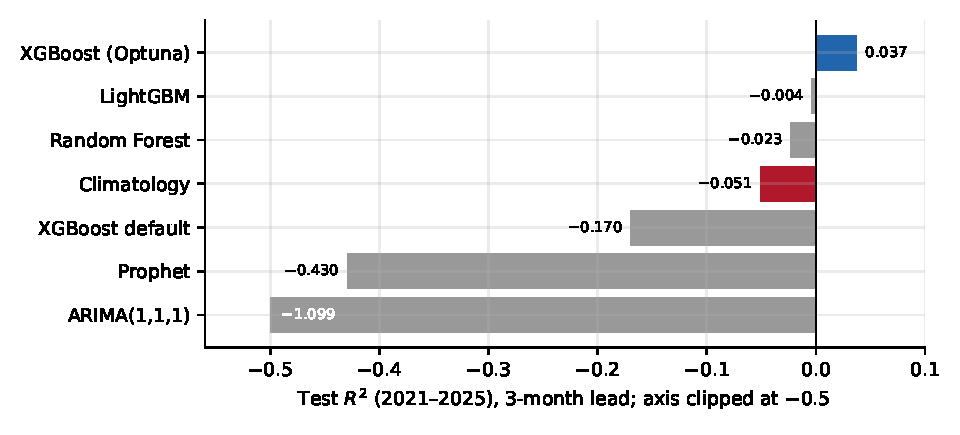
\includegraphics[width=0.85\textwidth]{figs_en/fig_bench.pdf}
\caption{Test $R^2$ by model in the leakage-free design. Only tuned XGBoost is positive, and its value is close to zero.}
\label{Fig:Bench}
\end{figure}

\subsection{Walk-forward validation results}
\label{SubSec:WFVres}

Table~\ref{Tab:WFV} gives the score of tuned XGBoost in each fold next to monthly climatology fitted on the same training window. XGBoost has the lower RMSE in folds 2, 3, and 5 and the higher RMSE in folds 1 and 4, and the mean RMSE is almost the same (0.0698 versus 0.0701). The fold $R^2$ of XGBoost ranges from 0.43 to 0.81, but climatology alone reaches 0.12 to 0.81, so these values mostly reflect seasonality and not ENSO skill.

\begin{table}[ht]
\centering
\caption{Walk-forward validation (five folds inside the training data). Months are counted in the training window and validation window of each fold. XGBoost uses the tuned hyperparameters; climatology is the mean SDCI per calendar month of the training window.}
\label{Tab:WFV}
\small
\begin{tabular}{rrrrrrrr}
\toprule
 & Train & Valid. & \multicolumn{3}{c}{XGBoost (tuned)} & \multicolumn{2}{c}{Climatology} \\
\cmidrule(lr){4-6}\cmidrule(lr){7-8}
Fold & months & months & RMSE & MAE & $R^2$ & RMSE & $R^2$ \\
\midrule
1 & 42 & 39 & 0.0839 & 0.0541 & 0.598 & 0.0718 & 0.706 \\
2 & 81 & 39 & 0.0602 & 0.0425 & 0.476 & 0.0778 & 0.124 \\
3 & 120 & 39 & 0.0382 & 0.0323 & 0.812 & 0.0389 & 0.805 \\
4 & 159 & 39 & 0.1148 & 0.0680 & 0.429 & 0.0994 & 0.572 \\
5 & 198 & 39 & 0.0520 & 0.0384 & 0.721 & 0.0628 & 0.592 \\
\midrule
\multicolumn{3}{l}{Mean RMSE} & \textbf{0.0698} & & & \textbf{0.0701} & \\
\bottomrule
\end{tabular}
\end{table}

\subsection{Reproducibility}
\label{SubSec:Repro}

In the initial design without a seed, five consecutive runs produced different best trials (numbers 31 to 49) and a test $R^2$ between 0.776 and 0.821, because the Optuna sampler is random. In the leakage-free R analysis with seed 42, two consecutive renders produced identical benchmark tables and 2026 projections. The figures reported here are therefore reproducible, whereas the initial figures (0.8044 in the notebook output and 0.8257 in the report) are not, because they came from unseeded runs. The Python notebook, which tunes with Optuna, gives a similar picture (tuned XGBoost test $R^2$ 0.037, climatology $-0.051$); the two tuning procedures find different hyperparameters, so the tuned values differ slightly, and in both cases the tuned model is close to zero.

\subsection{The 2026 Godzilla El Ni\~no scenario}
\label{SubSec:Scenario}

With the ONI path assumed to rise by 0.15 per month, ONI reaches about $+1.2$ in December 2026, a moderate El Ni\~no, not yet as strong as 2015. The quantile models project the lowest national SDCI in September 2026 at 0.399 with a 10--90\% range of 0.360--0.538. This is above the critical threshold of 0.3 but below the historical September mean (0.493); only 3 of the 26 observed Septembers (2002, 2015, and 2019) were lower. Because the model does not clearly beat climatology on the test months (Section~\ref{SubSec:ML}), the projection is a scenario-conditional indication of a drier-than-usual September, not a validated forecast of extreme drought.

%==================================
\section{Discussion}
\label{Sec:Discussion}

\paragraph{Target leakage is the main finding.} The difference between an $R^2$ of 0.80 and 0.07 comes entirely from one design decision: including variables that build the target. This agrees with the warning of Kaufman et al.\ \cite{kaufman2012leakage} that leakage is hard to notice precisely because the model scores look good. A quick check is to regress the target linearly on candidate predictors: an $R^2$ near 1 signals leakage. For a composite index, the practical rule is to treat the index components as part of the target.

\paragraph{ENSO gives a concurrent signal, not a three-month early warning.} The correlations and ONI coefficients are strongest at lead zero and vanish at leads of three months or more. This agrees with the picture that ENSO modulates Indonesian rainfall quickly through atmospheric circulation and local air--sea interaction \cite{hendon2003indonesian,aldrian2003rainfall}, rather than through a delay of several months. The effect is nonetheless small relative to the variation of the SDCI anomaly (maximum $R^2$ of 0.085), because most SDCI variation comes from seasonality (58.9\%) and other factors that are not modeled. As a result, an early-warning system relying only on ONI three months earlier gives no advantage over climatology.

\paragraph{Regional heterogeneity.} Java and Nusa Tenggara are the most sensitive and remain significant after multiple-testing correction, while Papua, Maluku, and Kalimantan are weak. This pattern agrees with regional rainfall differences reported earlier \cite{aldrian2003rainfall,hamada2002rainy}, but we did not test the cause. The national index averages eight regions with different sensitivities, so the national signal is weaker than that of the most responsive regions. Early warning focused on Java and Nusa Tenggara is likely more meaningful.

\paragraph{Usefulness of kinematic features.} ONI momentum and acceleration were designed to detect rapid warming before an El Ni\~no matures. On these data they gave no measurable advantage over climatology at a three-month lead. We did not test whether kinematic features help forecast ONI itself, which is a different goal.

\paragraph{Implications for early warning.} The results support using ENSO as a concurrent monitor and as context, and do not support the claim that a model trained on three-month-lagged ONI can warn of national drought. Improvements may come from additional predictors (for example the Indian Ocean Dipole, soil moisture, and persistence of the SDCI itself) and from regional targets.

\paragraph{Limitations.} (1) The target is a single national index averaged over eight regions. (2) There are only 312 months and 60 test months, so small differences between models cannot be distinguished from noise, and the Newey--West $p$-values are asymptotic. (3) Persistence of the SDCI (the lagged SDCI) was not tested as a predictor, although this benchmark is probably strong. (4) The ARIMA and Prophet benchmarks were not tuned. (5) The mean SDCI of the test period shifted from the training data (0.673 versus 0.610), which depresses the $R^2$ of every model. (6) The 2026 scenario depends on an assumed ONI path that only reaches $+1.2$, so it is not a simulation of an extreme El Ni\~no. (7) The SDCI formulation follows the project's definition; we did not compare it with other weightings. (8) Tuning uses random search instead of Bayesian optimization, so the tuned hyperparameters, and slightly the tuned scores, differ from the Python notebook run with Optuna.

%==================================
\section{Conclusion}
\label{Sec:Conclusion}

We tested how far ENSO predicts national drought in Indonesia using monthly data for 2000--2025. The initial design, which reported a test $R^2$ of about 0.80, turned out to leak: same-month NDVI, LST, and rainfall reconstruct the SDCI with a test $R^2$ of 1.000. After removing those components and lagging ENSO features by three months, tuned XGBoost reaches a test $R^2$ of only 0.070 (RMSE 0.0935), and monthly climatology $-0.051$ (RMSE 0.0993). The skill score of ONI against climatology is negative at leads of 1, 3, 6, and 9 months. ONI correlates negatively with the SDCI in the same month and the following month, most strongly in Java and Nusa Tenggara, but the relationship vanishes at leads of three months or more and explains less than a tenth of the anomaly variation. Under the linear-ONI scenario, the national SDCI for September 2026 is projected at 0.399 (10--90\% range 0.36--0.54), below the historical September mean of 0.493 but above the critical threshold of 0.3, without evidence that the model beats climatology. In practice, ENSO is suitable as a concurrent drought monitor for Java and Nusa Tenggara, but not as a sole predictor three months ahead. Checks for target leakage, a climatology benchmark, and a fixed seed should be standard practice in similar early-warning studies.

%==================================

\printbibliography[title={References}]

%==================================
\appendix

\section{Data and Code Availability}
\label{Sec:SuppA}

\sloppy
The monthly data (312 rows) are in \texttt{data/master\_dataset\_godzilla\_elnino\_2000\_2025.csv}. The R Markdown document \texttt{R/godzila-el-nino.Rmd} runs the full pipeline of the notebook \texttt{notebooks/godzila-el-nino.ipynb} in R (rendered output \texttt{R/godzila-el-nino.html}) and writes every reported model number to \texttt{R/hasil\_R.json}. The lead--lag statistics are in \texttt{R/analisis\_R.Rmd}. The script \texttt{artikel\_smds/buat\_figur.py} regenerates all figures from the data and \texttt{R/hasil\_R.json}, and recomputes the lead--lag tables with its own Newey--West implementation; the results match R for all leads. The seed used is 42.

\end{document}
